% Template for ICASSP-2026 paper; to be used with:
%          spconf.sty  - ICASSP/ICIP LaTeX style file, and
%          IEEEbib.bst - IEEE bibliography style file.
% --------------------------------------------------------------------------
\documentclass{article}
\usepackage{spconf,amsmath,graphicx,hyperref, pifont, multirow}

% Example definitions.
% --------------------
\def\x{{\mathbf x}}
\def\L{{\cal L}}

% Title.
% ------
\title{Streaming speech recognition with decoder-only large language models 
and latency optimization}
%
% Single address.
% ---------------
\name{Genshun Wan$^{\dagger 1}$, Wenhui Zhang$^{\dagger 2}$, Jing-Xuan Zhang$^{\star 3}$, Shifu Xiong$^1$, Jianqing Gao$^2$, Zhongfu Ye$^1$\thanks{
$\dagger$Equal contribution. $\star$Corresponding author.\\
This work was supported by the National Natural Science Foundation of China
(Grant No. 62401348), Fundamental Research Funds for the Central Universities (Grant No. GK202406005), Young Talent Fund of Association for Science and
Technology in Shaanxi, China (Grant No. 20250126).}}

\address{
$^1$University of Science and Technology of China, Hefei, P.R.China \\
$^2$iFLYTEK Research, iFLYTEK Co., Ltd., Hefei, P.R.China \\
$^3$School of Artificial Intelligence and Computer Science, 
Shaanxi Normal University, Xi'an, P.R. China \\
\small{\texttt{gswan@mail.ustc.edu.cn, whzhang9@iflytek.com, jxzhanggg@snnu.edu.cn}}
}
%
% For example:
% ------------
%\address{School\\
%	Department\\
%	Address}
%
% Two addresses (uncomment and modify for two-address case).
% ----------------------------------------------------------
%\twoauthors
%  {A. Author-one, B. Author-two\sthanks{Thanks to XYZ agency for funding.}}
%	{School A-B\\
%	Department A-B\\
%	Address A-B}
%  {C. Author-three, D. Author-four\sthanks{The fourth author performed the work
%	while at ...}}
%	{School C-D\\
%	Department C-D\\
%	Address C-D}
%
\begin{document}
\ninept
%
\maketitle
%
\begin{abstract}

%Recent studies have demonstrated the effectiveness of integrating large language models (LLMs) for automatic speech recognition (ASR). However, 
% While the success of integrating decoder-only large language models for automatic speech recognition (ASR),
% enabling streaming ASR  in such a framework remains a challenging and open question. 
% We propose a novel method for streaming LLM-based ASR. 
% A read/write policy network based on monotonic chunkwise attention (MoChA) is introduced to dynamically segment speech embeddings, which is interleaved with labels for training. During inference, incoming audio is buffered until the MoChA module triggers a read signal, at which point the buffered segment is fed into the LLM to predict output tokens. 
% This jointly optimization of our model and modular design naturally facilitates latency optimization. We introduce a minimal latency training loss to optimize the policy network for producing more accurate segmentation boundaries. Furthermore, we propose a joint training strategy in which a non-streaming LLM-ASR model and our streaming model share parameters.
% Experiments on the AISHELL-1 and AISHELL-2 Mandarin speech corpora show that our method outperforms recent streaming ASR baselines, while effectively controlling latency. Ablation studies confirm effective 
% of joint training and using of pretrained LLM parameters for ASR.
%Additional results verify the benefits of joint optimization between non-streaming and streaming models.

% Recent advances have demonstrated the potential of decoder-only large language models (LLMs) for automatic speech recognition (ASR). However, enabling streaming recognition within this framework remains a major challenge. In this work, we propose a novel streaming ASR approach that integrates a read/write policy network with monotonic chunkwise attention (MoChA) to dynamically segment speech embeddings. These segments are interleaved with label sequences during training, allowing seamless integration with the LLM. During inference, the audio stream is buffered until the MoChA module triggers a read signal, at which point the buffered segment together with the previous token is fed into the LLM for the next token prediction.
% We also introduce a minimal-latency training objective to guide the policy network toward accurate segmentation boundaries. Furthermore, we adopt a joint training strategy in which a non-streaming LLM-ASR model and our streaming model share parameters.
% Experiments on the AISHELL-1 and AISHELL-2 Mandarin benchmarks demonstrate that our method consistently outperforms recent streaming ASR baselines, achieving character error rates of 5.1\% and 5.5\%, respectively. The latency optimization results in a 62.5\% reduction in average token generation delay with negligible impact on recognition accuracy. 

Recent advances have demonstrated the potential of decoder-only large language models (LLMs) for automatic speech recognition (ASR). However, enabling streaming recognition within this framework remains a challenge. In this work, we propose a novel streaming ASR approach that integrates a read/write policy network with monotonic chunkwise attention (MoChA) to dynamically segment speech embeddings. These segments are interleaved with label sequences during training, enabling seamless integration with the LLM. During inference, the audio stream is buffered until the MoChA module triggers a read signal, at which point the buffered segment together with the previous token is fed into the LLM for the next token prediction.
We also introduce a minimal-latency training objective to guide the policy network toward accurate segmentation boundaries. Furthermore, we adopt a joint training strategy in which a non-streaming LLM-ASR model and our streaming model share parameters.
Experiments on the AISHELL-1 and AISHELL-2 Mandarin benchmarks demonstrate that our method consistently outperforms recent streaming ASR baselines, achieving character error rates of 5.1\% and 5.5\%, respectively. The latency optimization results in a 62.5\% reduction in average token generation delay with negligible impact on recognition accuracy.
 % Ablation studies further confirm the effectiveness of joint training and the benefit of leveraging pretrained LLM parameters for streaming ASR.



\end{abstract}
%
\begin{keywords}
automatic speech recognition, streaming ASR, large language models, latency
\end{keywords}
%
\section{Introduction}
\label{sec:intro}


Streaming automatic speech recognition (ASR), also referred to as online ASR, aims to transcribe speech incrementally in real time. It plays a crucial role in practical applications such as live captioning for online meetings and simultaneous translation. A large body of research has explored streaming ASR within conventional end-to-end frameworks, typically relying on unidirectional or blockwise encoders combined with connectionist temporal classification (CTC)~\cite{10.1145/1143844.1143891}, recurrent neural network transducers (RNN-T)~\cite{6638947}, or Transformer transducers~\cite{9053896}. 
% Both CTC and transducer models employ frame-synchronous decoding, making them naturally suitable for streaming scenarios. 
In parallel, researchers have also investigated attention-based encoder–decoder (AED) architectures, which adopt label-synchronous decoding. To enable streaming in AED models, several methods have been proposed, including triggered attention~\cite{8683510}, monotonic attention~\cite{10.5555/3305890.3305974}, monotonic chunkwise attention (MoChA)~\cite{chiu2018monotonic}, and its subsequent extensions~\cite{arivazhagan-etal-2019-monotonic, inaguma2020enhancing}.

% Streaming ASR, also known as online ASR, aims to transcribe the audio in real time incrementally. 
% Streaming ASR is vital for practice real-time scenarios, such as subtitle generation during online meeting.
% Many studies have investigated to achieve the streaming ASR under the
% conventional end-to-end speech recognition models, including 
% unidirectional or blockwise processing encoders~\cite{8462497,9003749} combined with
% connectionist temporal classification (CTC)~\cite{10.1145/1143844.1143891, pmlr-v48-amodei16}, RNN transducer~\cite{6638947,8268935}, or Transformer transducer~\cite{9053896}.
% CTC and transducers adopt frame-synchronous decoding, which is suitable for streaming ASR.
% On the other hand, researcher also explore streaming ASR with attention-based encoder-decoder (AED) models, which adopt label-synchronous decoding.
% Methods are proposed such as triggered attention~\cite{8683510}, monotonic attention~\cite{10.5555/3305890.3305974}, 
% monotonic chunkwise attention~\cite{chiu2018monotonic} (MoChA) and its extensions~\cite{arivazhagan-etal-2019-monotonic, inaguma2020enhancing}.


% Recent year have witness rapid development of large language models (LLM) and
% its applications for multimodal information process~\cite{xu2025qwen25omnitechnicalreport, 10.5555/3692070.3693991, zhan-etal-2024-anygpt}.
% With the rapid development of large language models~\cite{xu2025qwen25omnitechnicalreport, 10.5555/3692070.3693991},
% leveraging decoder-only LLM for effective speech recognition have also attract much attention~\cite{10447553, maiti2024voxtlm, wang-etal-2024-exploring, fathullah2024prompting}.
%  Despite the success of intergating LLMs for ASR in 
%  non-streaming scenarios, the achieving streaming ASR
% with a decoder-only LLM remains an open question.
% Tsunoo et al.~\cite{tsunoo24_interspeech} proposed 
% a blockwise streaming LLM-based ASR with CTC compression,
% where the LLM estimates the output tokens promptly at each
% block.
% Jia et al.~\cite{10890853} proposed SpeechLLM-XL, which process 
% audio and text into fix-sized chunks using a CTC force alignment model for 
% streaming speech recognition.
% BESTOW~\cite{10832146} combines GPT-style and T5-style architecture,
% implement a wait-k strategy for streaming ASR.
% Chen et al.~\cite{chen24u_interspeech} proposed a text token insertion (TTI) and boundary token insertion model (BTI)
% for LLM-based ASR with discrete speech tokens,  where the boundary of speech is first extracted from a hybird ASR method.
% The previous studies  requires either a CTC or a hybird model
% to extract the audio and text force alignment in advance, 
% this cascade method lead the end-to-end optimization difficult.
% Also, for the method adopts the strategy that generates
% tokens after a fix-size audio chunk for streaming recognition,
% minimizing the latency for token generation adaptively is difficult to be achieved.

With the rapid development of large language models (LLMs), leveraging decoder-only architectures for speech recognition has recently attracted considerable attention~\cite{10.5555/3692070.3693991, 10447553, wang-etal-2024-exploring, fathullah2024prompting}. While LLMs have shown remarkable success in non-streaming ASR scenarios, extending them to streaming recognition remains an open challenge. Tsunoo et al.~\cite{tsunoo24_interspeech} proposed a blockwise streaming LLM-based ASR framework with CTC compression, where the LLM predicts output tokens after each block. Jia et al.\cite{10890853} introduced SpeechLLM-XL, which processes speech and text into fixed-size chunks using a CTC force-alignment model for streaming recognition. BESTOW~\cite{10832146} combines GPT-style and T5-style architectures and implements a wait-k strategy for streaming ASR. Chen et al.~\cite{chen24u_interspeech} proposed text token insertion (TTI) and boundary token insertion (BTI) models for LLM-based ASR with discrete speech tokens, where speech boundaries are first extracted using a hybrid ASR system.
Despite these efforts, existing approaches often rely on CTC or hybrid models to perform forced alignment between speech and text in advance. Such cascaded designs complicate end-to-end optimization. Moreover, methods that generate tokens only after fixed-size audio chunks face inherent limitations in adaptively minimizing token-generation latency during streaming recognition.


In this work, we propose a streaming LLM-based ASR method. Our method employs a read/write policy network based on monotonic chunkwise attention (MoChA), which is used for adaptively segmenting the incoming speech before passing it to the LLM for text prediction. Specifically, the MoChA module monitors speech embeddings frame by frame until a read signal is triggered; at that point, the buffered embeddings and the previous token are fed into the LLM to decode the next token. During both training and inference, the audio and text embeddings are interleaved to enable synchronized processing.
For streaming audio encoding, we adopt context-sensitive chunking~\cite{an22_interspeech} with a speech encoder. The encoder outputs are projected through an adaptor and then provided to the LLM as prompts. Owing to the modularized design of the policy network for audio reading, we further apply a minimal latency training (minLT) loss~\cite{inaguma2020minimum}, which effectively reduces the latency of streaming recognition.
The LLM is trained jointly with the speech encoder, policy network, and adaptor using low-rank adaptation (LoRA)~\cite{hu2022lora} in an end-to-end manner. We also propose parameter sharing and joint optimization between the streaming and non-streaming ASR models. This unified approach simplifies the training pipeline and reduces the overall development cost of ASR systems.
% while ensuring consistency across both streaming and non-streaming scenarios.
% In this work, we proposed a streaming LLM-based ASR model, in which
% a read/write policy network based on MoChA is employed to
% guide the adaptive segmentation of
% audio, which is then fed into the LLM for text prediction.
% Specifically, the MoChA module inspect the audio embeddings frame-by-frame until triggering a read operation, and then the buffered audio embedding are feed into LLM for decoding a token, then waiting
% for the next triggering.
% The audio embeddings sequence and text embeddings are interleaved during training and testing.
% We use contextual sensitive chunking~\cite{an22_interspeech} for the the streaming encoding 
% of audio using the speech encoder. The output of the speech encoder
% is projected by an adaptor then pass to the LLM as prompt.
% Thanks to the modularization of policy network for controling
% the audio reading, we further employ a minimal latency training (minLT) loss~\cite{inaguma2020minimum} on it, which  help reducing the latency of the streaming LLM-based ASR effectively.
% The large language model is trained with low-rank adaptation technique, joint with the audio encoder, policy network and 
% the adaptor, in an end-to-end manner.
% We also explore the full parameter sharing and joint optimization of 
% the streaming and non-streaming model. Unifiying the non-streaming and streaming model
% method simplifies the workflow and the cost of training and development of ASR models.

% We conduct experiments on two widely-used Mandarin Corpra, AISHELL-1 and AISHELL-2.
% The experiment shows that our method outperform the recent proposed baseline streaming LLM-ASR method. 
% The the employment of minimal latency training effectively reduces 
% the training latency. 
% And the sharing parameters and joint training both
% non-stream and stream model shows no degradation compared to training them separately. 
% Our ablation study also confirmed effectiveness of several key components in our method.


We conduct experiments on two widely used Mandarin corpora, AISHELL-1 and AISHELL-2, as well as an in-house multi-domain dataset. The results demonstrate that our method consistently outperforms recently proposed baseline streaming LLM-ASR systems. Incorporating minimal latency training (minLT) effectively reduces recognition delay while maintaining competitive accuracy. Furthermore, ablation experiments confirm the effectiveness of our unified streaming and non-streaming framework and demonstrate the benefits of leveraging pretrained LLM parameters.



\section{Related Works}

%\section{Related Works}

Recent studies on LLM-based ASR focus on enhancing speech recognition by leveraging LLMs’ in-context learning~\cite{10447553}, world knowledge~\cite{wang-etal-2024-exploring}, and instruction-following capabilities~\cite{instruction-following-speech}.  
LLM-based ASR systems typically adopt either discrete~\cite{zhang-etal-2023-speechgpt, chen2024loss} or continuous audio representations~\cite{10447553, wu2023decoder, fathullah2024prompting, 10446898}.  
The discrete-token approach, such as SpeechGPT~\cite{zhang-etal-2023-speechgpt}, employs a speech tokenizer model~\cite{hsu2021hubert,zhang2024speechtokenizer} to quantize speech into discrete units, which are then merged with the LLM vocabulary.  
In contrast, methods using continuous audio embeddings~\cite{fathullah2024prompting} rely on a pretrained audio encoder, with its output representations optionally compressed via strided CNNs~\cite{fathullah2024prompting}, frame pooling~\cite{ma2024embarrassingly}, Q-formers~\cite{10445874}, or CTC-based compressors~\cite{wu2023decoder}. The resulting audio embeddings are projected into the LLM word embedding space to prompt transcription.  
Typically, continuous embeddings are treated as soft prompts that are prepended to the label embeddings before being fed into LLMs. Other works adopt a Flamingo-style~\cite{alayrac2022flamingo} integration, where audio features are injected through cross-attention modules to fuse them with the input embeddings or hidden representations of LLMs~\cite{10832146, radhakrishnan-etal-2023-whispering}.  
% Previous work has demonstrated the effectiveness of adapting pretrained LLMs to speech recognition tasks. However, most studies have primarily focused on non-streaming ASR.  
Our work investigates streaming ASR under the widely used configuration of LLM-based ASR, which employs continuous speech embeddings as soft prompts. 
%This approach has been shown to yield strong ASR performance in prior studies, and we extend it to the streaming setting.


% Recent study of LLM-based ASR focus on improving or extend the speech recognition ability by leveraging LLM's in context learning~\cite{10447553}, world knowledge~\cite{wang-etal-2024-exploring}, or 
% instruction following ability~\cite{instruction-following-speech}.
% The LLM-based ASR can use either discrete~\cite{maiti2024voxtlm, zhang-etal-2023-speechgpt, chen2024loss} or continuous audio representations~\cite{10447553, wu2023decoder, fathullah2024prompting, 10446898}.
% The former approach, such as SpeechGPT~\cite{zhang-etal-2023-speechgpt}, usually employ a speech tokenizer model~\cite{hsu2021hubert,zhang2024speechtokenizer}
%  to quantize the speech into discrete tokens, which is then
% merged with the vocabulary of LLMs. 
% The method employ continuous audio embedding~\cite{fathullah2024prompting} typically
% employ a pretrained audio encoder, the output representation of which is then  optionally temprally compressed such as 
% a strided CNN~\cite{ fathullah2024prompting}, pooling consective frame~\cite{ma2024embarrassingly}, Q-former~\cite{10445874}, or a CTC compressor~\cite{wu2023decoder}.
% Then the audio embedding are project to the word embedding space of LLMs to prompt the
%  LLM to transcribe the text.
% The continous audio embedding is typicaly adopts as soft prompt
% be fed into LLMs, prepending it with the label embeddings.
%  other work alternatively employ 
%  a Flamingo-style~\cite{alayrac2022flamingo} audio injection into LLMs, which
%  use cross-attention module to fuse the audio
%  embedding with the input embeddings or hidden
%  representations of LLMs~\cite{10832146, radhakrishnan-etal-2023-whispering, li24b_interspeech}.
 
% The previous work have shown the effectiveness of transferring
%  a pretrained LLM to speech recognition task,
%  However, most of them focus only on non-streaming ASR.
%  Our work explore the stream ASR, using the most popular configuration of
%  LLM-based ASR, which adopts continues speech embeddings and using
% it as soft prompt to LLMs, which have been demonstrated its effectiveness and strong ASR performance in previous studies.


\begin{figure}
    \centering
    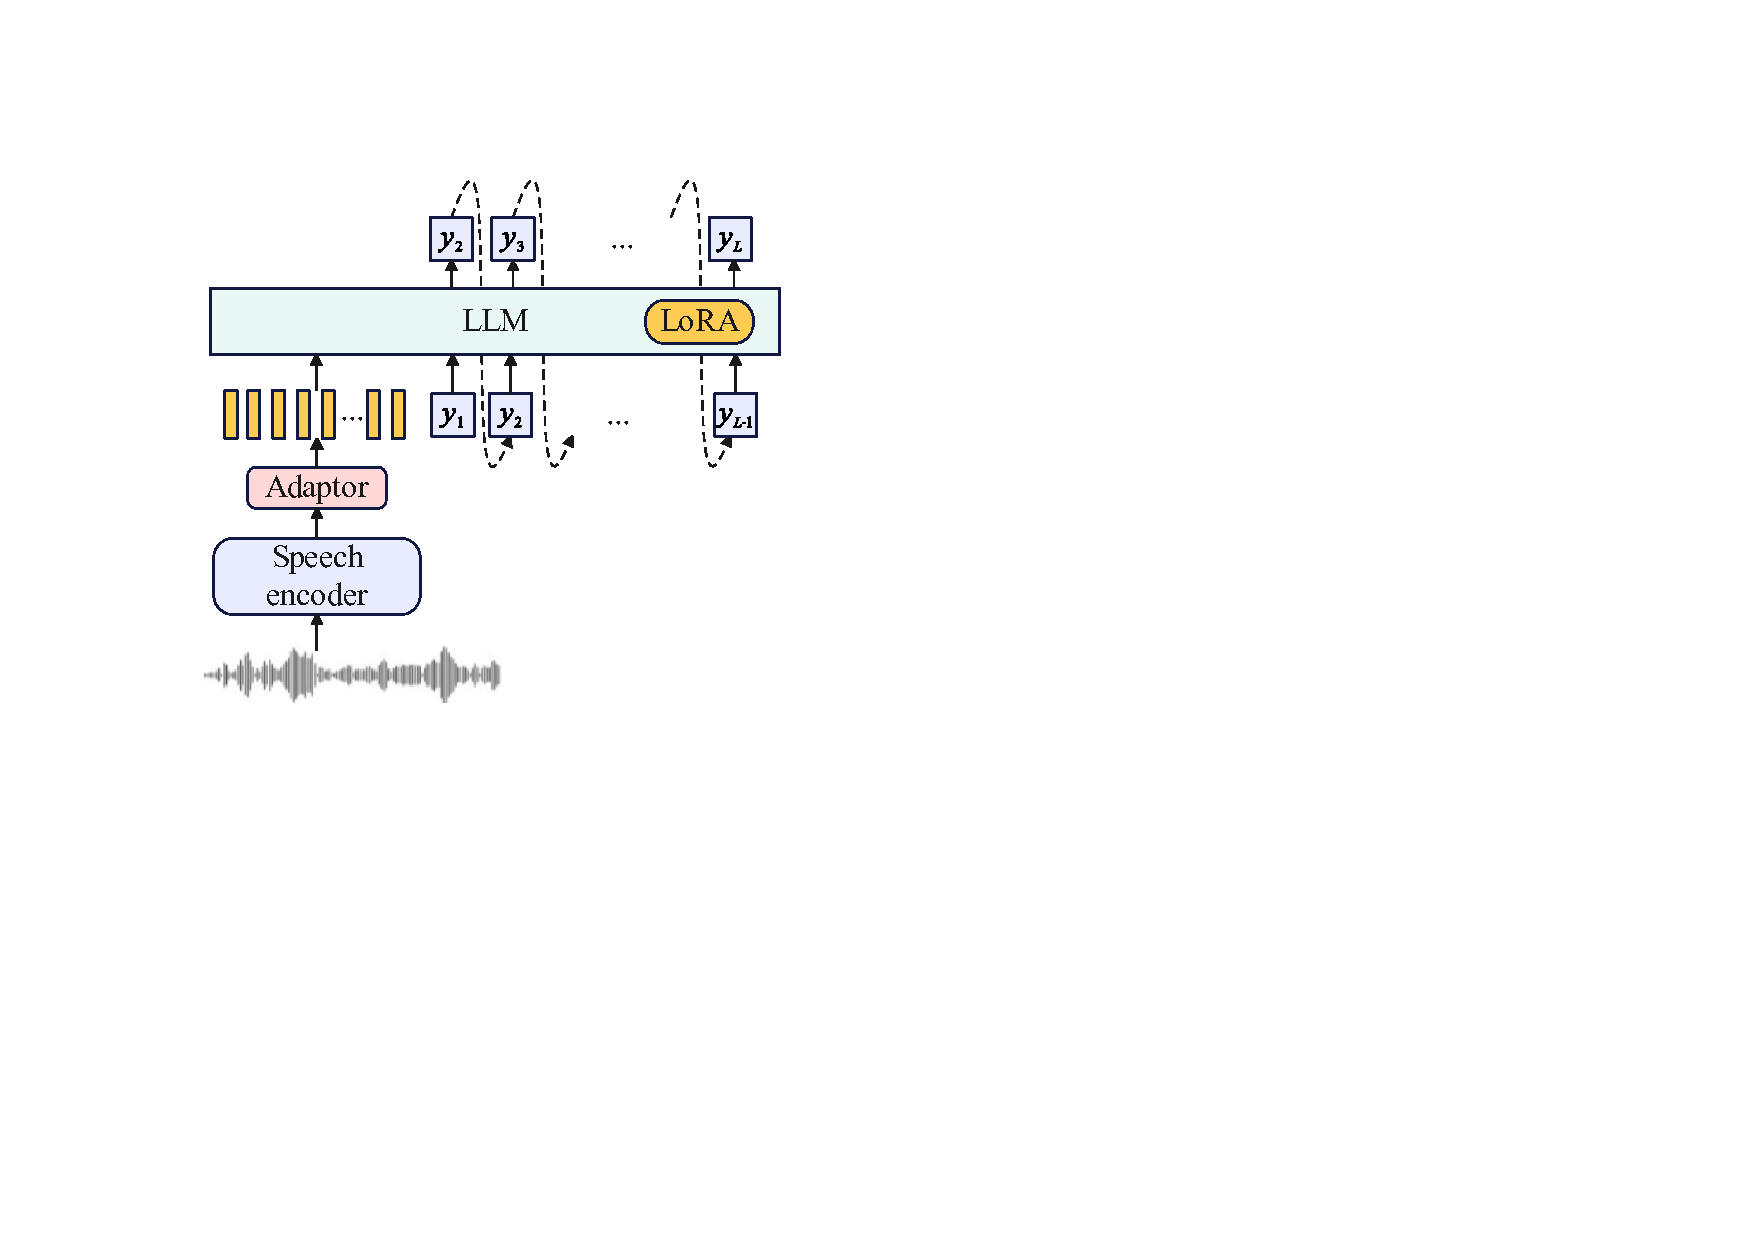
\includegraphics[width=0.75\linewidth]{figure1.pdf}
    \caption{Non-streaming LLM-based ASR architecture. $y_1$ and $y_L$
    represent the BOS and EOS token, respectively.}
    \label{fig:fig1}
\end{figure}




\section{Non-streaming LLM-based ASR}

%\section{Non-streaming LLM-based ASR}

The architecture of a non-streaming LLM-based ASR model~\cite{fathullah2024prompting, ma2024embarrassingly} is illustrated in Figure~\ref{fig:fig1}.  
The model employs a speech encoder to transform the input speech $X$ into speech representations.  
% In our implementation, we adopt a Conformer-based encoder due to its strong performance in speech modeling.  
An adaptor module is then used to project the audio representations into the word embedding space of the LLM.  
Following prior work~\cite{ma2024embarrassingly}, we implement the adaptor as a feed-forward network, which offers both simplicity and competitive performance in ASR tasks.  
The converted audio prompt tokens $h_{1:N}$ are subsequently fed into a decoder-only LLM to generate the corresponding transcription.  
Formally, the conditional probability of the text sequence given the speech input is estimated as
\begin{equation}
    P(Y | X) = \prod_{i=2}^{L} P(y_{i} \mid h_{1:N}, y_{1:i-1}, \theta_{LLM}),
\end{equation}
where $\theta_{LLM}$ denotes the parameters of the LLM.  $y_1, \dots, y_L$
represents the label sequence, where $y_1$ and $y_L$ are special begin of sentence (BOS) and
end of sentence (EOS) token.
The pretrained LLM is commonly equipped with low-rank adaptation (LoRA)~\cite{hu2022lora} weights, enabling memory-efficient finetuning.  
During training, given paired speech–text samples, the model is optimized using a cross-entropy loss to maximize the log-likelihood of the target text sequence.  
The loss is masked over the audio prompt tokens to ensure that only the textual part contributes to optimization.  
At inference time, the input speech is first fully encoded into hidden representations, after which the LLM generates the output text autoregressively until an EOS token is produced.


% The architecture of a non-stream LLM-based ASR model~\cite{fathullah2024prompting, ma2024embarrassingly} is illustrated in Figure~\ref{fig:fig1}. It employs a
% speech encoder to process the speech input $X$ into
% audio representations. 
% We adapt a speech encoder based on the Conformer architecture.
% Then an adaptor component is then adopted for converting the audio representations into the space of word embeddings of LLMs. 
% We adopt a feed forward network for the adaptor because its simplicity and competitive performance in ASR task~\cite{ma2024embarrassingly}.
% Then the converted audio prompt tokens $h_{1:N}$ is fed into a decoder-only LLM for transcribing the corresponding text.
% %for decoding the text autoregressively. 
% The conditional probability of text sequence given speech input is estimated by the LLM as
% \begin{equation}
%     P(Y | X) = \prod_{i=1}^{L} P(y_i | h_{1:N}, y_{1:i-1}, \theta_{LLM}),
% \end{equation}
% where $\theta_{LLM}$ represents the parameters of LLM.
% The pretrained LLM is usually augmented with low-rank adaptation (LoRA)~\cite{hu2022lora} weights 
% for memory-efficient finetuning. During training, given
% paired speech and label samples, 
% the cross-entropy loss is adopted for maximizing the
% log-likelihood of the label text sequence. The loss is mask out for the
% the  audio prompt input sequence.
% During inference, the input speech is first converted into hidden representations at once. Then, the text is generate auto-regressively until decoding
% an end-of-sentence (EOS) token.
%During training, the LLM is us

\begin{figure}
    \centering
    
\includegraphics[width=0.76\linewidth]{figure2.pdf}
    \caption{Our proposed streaming LLM-based ASR architecture. $y_1$ and $y_L$
    represent the BOS and EOS token, respectively.}
    \label{fig:fig2}
\end{figure}


\section{Proposed Method}
\subsection{Model architecture}

% For streaming speech encoding, we use a  context sensitive chunking technique following previous study~\cite{an22_interspeech}. 
% Specifically, audio are chunked into segments with a past and
% a future context window. Then the Conformer speech encoder is used to process each audio chunks in parallel during training. After discarding outputs from the context frames, outputs from those chunks are then spliced to recover the utterance-level audio representations.
% Despite introducing some extra computation and latency,
% context sensitive chunking can effectively improve the
% streaming recognition performance.
% The speech embeddings is then transformed by
% the adaptor,
% which is fed into the LLM for streaming text decoding.
%  A read/write policy network is introduced for acquiring the
% alignment between text and speech, which is then used to  segment the speech input adaptively, as illustrated in Figure~\ref{fig:fig2}.

For streaming speech encoding, we adopt a context-sensitive chunking strategy following prior work~\cite{an22_interspeech}.
The input audio is segmented into chunks, each with an additional history context window. We avoid using any future context to prevent additional encoding latency.
During training, these chunks are processed in parallel by a Conformer-based speech encoder. After discarding the outputs corresponding to the context frames, the remaining chunk-level representations are concatenated to reconstruct the utterance-level audio features.
% Although this approach introduces extra computation and latency, it significantly improves the recognition performance in the streaming setting.
The resulting speech embeddings are then transformed by an adaptor module into the representation space of the LLM. 
%These transformed embeddings are fed into the decoder-only LLM for streaming text prediction.
To further align speech and text sequences, we introduce a read/write policy network that adaptively segments the incoming speech stream. This policy enables dynamic synchronization between audio input and text output, as illustrated in Figure~\ref{fig:fig2}.



Our read/write policy network is built upon monotonic chunkwise attention (MoChA)~\cite{chiu2018monotonic}, operating with a lightweight decoder.
At each decoder timestep $i$, the attention mechanism begins scanning the encoder outputs starting from the previously attended position $t_{i-1}$.
A selection probability $p_{i,j}$ is computed for each encoder frame. Once this probability exceeds a predefined threshold at frame $j$, the model triggers a stop-and-decode signal and sets $t_i = j$.
To enhance flexibility, MoChA applies an additional soft chunkwise attention over the hard alignment, allowing the decoder to aggregate information within a local region.
This process generates an encoder index sequence $[t_1, \dots, t_{L}]$ that aligns synchronously with the output tokens $[y_2, \dots, y_L]$, where $t_1=0$.
Intuitively, each token $y_{i}$ for $i=\{2,\dots,L\}$ is decoded based on the acoustic segment $h_{t_{i-1} + 1:t_i} = [h_{t_{i-1} + 1}, \dots, h_{t_i}]$,  which contains the minimal speech context necessary for predicting $y_{i}$.

As shown in Figure~\ref{fig:fig2}, the alignment produced by the policy network is used to interleave segmented speech embeddings with the corresponding text sequence:
\begin{equation}
H_y = [ h_{t_1+1:t_2}, y_1, h_{t_2+1:t_3}, y_2, \dots, h_{t_{L-1}+1:t_{L}}, y_{L-1} ] .
\end{equation}
The resulting mixed sequence $H_y$ is then fed into the LLM during training.
Accordingly, the conditional probability of the text sequence is modeled as:
\begin{equation}
P(Y|X) = \prod_{i=2}^{L} P(y_{i} | h_{t_1+1:t_2}, y_1, \dots, h_{t_{i-1}+1:t_i},  y_{i-1}, \theta_{LLM}) .
\end{equation}
The cross-entropy loss $L_{LLM}$ is only computed at the final frame of each segment, where the next token $y_i$ is predicted.
Our policy network and LLM are trained jointly, enabling dynamic refinement of the segmentation boundaries as training progresses.
%With convergence, or with the aid of external alignment regularization, the boundary predictions become more reliable. Consequently, the LLM can adapt to the segmented acoustic patterns while maintaining high streaming recognition accuracy.


% Our read/write policy network is based on the monotonic chunkwise attention (MoChA)~\cite{chiu2018monotonic}, which works with a small
% decoder.
% Specifically, at each decoder output timestep $i$, 
% the attention mechanism begins inspecting the encoder output entries starting at the encoder index it 
% attended to at the previous output timestep, 
% referred to as $t_{i-1}$.
% it introduce a selection probability $p_{i, j}$
% When the selection probability surpass a predefined threshold
% at the $j$ frame of the encoder output,
% the model trigger a
% stop and decoding signal, and then sets $t_i = j$.
% MoChA attention further use a additional soft chunkwise attention on the hard alignment to increase its modeling flexibility and capacity. In summary, MoChA attention
%  generates a encoder time index sequence $[t_0, t_1, t_2 , \dots, t_L]$, which is synchronous with
% the decoding labels $[y_1, y_2, \dots, y_L]$, where $t_0 = 1$. The encoder time index sequence segment
% audios between $t_{i-1}$  and $t_i$ that necessary for decoding the correponding text token $y_i$.

%  As shown in Figure~\ref{fig:fig2}, alignment between text and speech provided by the policy network is utilized to
% split speech embeddings into segments, then interleaved with the text as  
% \begin{equation}
%    H_y = [ h_{t_0:t_1}, y_1, h_{t_1+1:t_2}, y_2, \dots, h_{t_{L-1}+1:t_L}, y_L]
% \end{equation}
% Then, the mixed sequence $H_y$ is fed into LLM for training.
% Therefore, the LLM models probability of text labels as 
% \begin{equation}
% P(Y|X) = \prod_{i=1}^L P(y_i | h_{t_0:t_1}, y_1, \dots, y_{i-1} , h_{t_{i-1}+1:t_i}, \theta_{LLM})
% \end{equation}
% The cross-entropy loss $L_{LLM}$ is only computed at the last frame of each audio segment, where the next text token is predicted.
% Our policy network and LLM are trained jointly. 
% During training, the boundary of audio segments from the  MoChA attention 
% may improve as the model converages, or by introducing regularization 
% from extra alignment information. Therefore, the LLM
% can adapt to the audio segments pattern while maintaining high accuracy of streaming ASR.


\subsection{Training strategy}

The LLM output is optimized with a standard cross-entropy loss $L_{LLM}$.
In addition, the small decoder within the policy network is trained using a cross-entropy loss $L_{MoChA}$, with the same vocabulary as the LLM.
It is important to note that the policy network output is only used during training and discarded at inference.

To further reduce latency, we incorporate a minimal latency training (minLT) loss $L_{minLT}$.
An HMM-based hybrid ASR system is first employed to generate force alignments between speech and text.
Following prior work~\cite{inaguma2020minimum}, we adopt a differentiable expected latency objective:
\begin{equation}
L_{minLT} = \frac{1}{L}\sum_{i=2}^L \sum_{j=1}^N | j \alpha_{i, j} - b_i |,
\end{equation}
where $\alpha_{i,j}$ is the marginalized alignment probability from MoChA, and $b_i$ is the gold boundary from the forced alignment.
The overall training objective is thus:
\begin{equation}
L_{total} = L_{LLM} + L_{MoChA} + \lambda L_{minLT},
\end{equation}
where $\lambda$ is a hyperparameter that balances the latency regularization term.

For efficient fine-tuning of the LLM, we adopt LoRA parameters.
The speech encoder, adaptor, and policy network are trained jointly with LoRA-based optimization from scratch.
Moreover, we propose a joint training scheme that integrates both streaming and non-streaming ASR.
The two models share all parameters but differ in the forward computation path.
During training, each batch is randomly assigned to either the streaming or non-streaming mode, allowing the model to learn both tasks simultaneously.

% \subsection{Training strategy}
% The output of LLM is trained with a cross-entropy loss $L_{LLM}$.
% Additionally, 
% the outputs of the  small decoder within the policy network is trained with
% a cross-entropy loss $L_{MoChA}$, where
% the  same vocabulary as the LLM's is adopted.
% It's worth to notice that the output of policy network
% is not used during inference.


% To optimize the latency, a minimal latency training loss $L_{minLT}$ is further used.
% A HMM-based hybird ASR model is first used to generate force alignment 
% between audio and text. Follow the previous research~\cite{inaguma2020minimum},
% a differentiable
% expected latency objective is adopted as
% \begin{equation}
%     L_{minLT} = \frac{1}{L}\sum_{i=1}^L | \sum_{j=1}^N j\alpha_{i, j} - b_i|,
% \end{equation}
% where $\alpha_{i, j}$ is marginalized probability of alignment in MoChA, $b_i$ is gold boundary from
% the force alignment.
% In summary, our model is trained with a total loss as 
% \begin{equation}
%     L = L_{LLM} + L_{MoChA} + \lambda L_{minLT},
% \end{equation}
% where $\lambda $ is a hyper-parameter controls the weighting of latency optimization loss.

% During training, the LLM is introduced with low-rank adaptation parameters
% for efficient finetuning. The speech encoder, adaptor, and the policy network is
% trained jointly with LoRA parameters from scratch.
% We also proposed to train our streaming LLM-based ASR method jointly with the full-context
% non-streaming model. Both model shares all  parameters, only
% pass through different operations during forward process. During training, we randomly 
% decide the usage of each batch of data  for optimizing streaming or non-streaming ASR task.
%As shown in our experiments in Section~\ref{sec:subsecab}, this strategy leads to no performance degradation.

\subsection{Inference}
During inference, the input speech is first encoded and processed into chunk-level representations.
The policy network then scans these representations until a selection signal is triggered.
Once triggered, the buffered audio segment together with the previous token is passed to the LLM, which generates the next token.
The predicted token is subsequently fed back into both the LLM and the MoChA attention module of the policy network.
This process is repeated iteratively until the LLM outputs an EOS token, completing the transcription.

% \subsection{Inference}
% During inference, our proposed method first encoding and processing chunkwise audio input into audio representations. 
% the policy network inspect the audio input until
% it triggers a selection signal. Then the buffer audio input are fed into LLM for
% decoding a token. The predicted token is then feedback into input of both LLM and MoChA attention module
% in the policy network, which is continue until a end of sentence (EOS) token is decoded by LLM.
%We also implement a beam search version for this decoding process.

\section{Experiments}
\subsection{Experiments configuration}
We evaluate our proposed method on three Mandarin datasets: AISHELL-1, AISHELL-2, and a multi-domain in-house dataset (MD).
AISHELL-1~\cite{bu2017aishell} 
 consists of 165 hours of speech (120k/14k/7k utterances for training, development, and testing, respectively).
AISHELL-2\footnote{\url{https://github.com/kaldi-asr/kaldi/blob/master/egs/aishell2}}
 provides 1,000 hours of training data, along with a development set of 2,500 utterances and a test set of 5,000 utterances.
The MD dataset contains roughly 1 hour of speech collected from multiple domains, such as finance, education, and film, and is used exclusively for evaluation.

Our speech encoder is a 12-layer Conformer with 8 attention heads, a hidden dimension of 512, and a feed-forward dimension of 2048. For streaming encoding, we adopt a chunk size of 0.4s, with left context windows of 1.6s. The adaptor is a feed-forward network with a hidden dimension of 1024 and GELU activation.
The LLM is initialized from pretrained Qwen 2.5-1.5B, which consists of 28 Transformer blocks, 12 attention heads, and a hidden dimension of 1536. We retain the original tokenizer and vocabulary to mitigate catastrophic forgetting compared with reinitializing embeddings. Low-rank adaptation (LoRA) weights are applied to the query, key, value, and output projection of the attention modules, with a rank of 32 and scaling factor $\alpha = 64$. The minimal latency (minLT) loss weight $\lambda$ is set to 0.1.

For optimization, we use AdamW with a triangular cyclic learning rate scheduler, which significantly accelerates convergence. The maximum and minimum learning rates are set to $1.5 \times 10^{-4}$ and 0, respectively, with each cycle spanning 25k updates for a total of 100k training steps. During inference, beam search with a beam size of 10 is adopted. 
%All experiments are implemented using Fairseq.
%\footnote{\url{https://github.com/facebookresearch/fairseq}}.

% 
% We use three datasets in our experiments, including AISHELL-1,
% AISHELL-2, and a multi-domain in-house dataset (i.e., MD).
% AISHELL-1\footnote{\url{https://openslr.org/33/}} contains 150/10/5 hours Mandarin speech with 120k/14k/7k utterances for training/development/test dataset.
% AISHELL-2\footnote{\url{https://github.com/kaldi-asr/kaldi/blob/master/egs/aishell2/}} contains 1000 hours with around 1 million utterances
% for training, additional development and test set with 2500 and 5000 utterances are also provided.
% MD dataset is an in-house Mandarin dataset used for evaluation purpose, which contains around 1 hours speech covering 
% multi-domain speech, such as financial, education, movie and so on.


% Our speech encoder employ a 12-layer Conformer, which has
% a 8 attention heads, 512 hidden dimension, and 2048 feed foward dimension.
% For streaming encoding, we used a chunk size of 0.4s for audio
% chunking, with a past and future context window of 0.16 and 0.08s, respectively.
% The adoptor use a feed-forward network with 1024 hidden dimension 
% and GELU activation.
% We use pretrained Qwen 2.5-1.5B for intialization the parameters
% of LLM, which contain 28 Transformer blocks, 12 attention heads and a hidden dimension of 1536.
% We inherit the same vocabulary size and the tokenizer of pretrained LLM. Our initial experiments showed that
% this help to prevent the knowledge forgetting of LLM
% compared to replace with a new tokenizer and embedding layer of LLM.  We add LoRA weights to the query, key, value, and dense
% projection of attention module in the LLM, with a LoRA rank of 32 and  multiply scaler $\alpha$ of 64. The minLT loss weight $\lambda$ is set to 0.1.

% We used AdamW optimizer during training.
% A triangular cyclic learning rate schedular was adopted,
% which help to accelerate the convergence speed significantly.
% The maximum and minimum learning rate is $1.5\times 10^{-4}$ and 0, respectively. A cycle spans over 25k updates for a total of 100k training updates of our model.
% For testing, we used 
% the beam search strategy with of beam size of 10. Our method was
% implemented with Fairseq~\footnote{\url{https://github.com/facebookresearch/fairseq}}.



\subsection{Comparison with baselines}


\begin{table}
   \caption{Character error rates of different methods on the testset of AISHELL-1. $^{\dagger}$Our reproduction results.}
    \label{tab:tab1}
    \centering
    \begin{tabular}{c c c c }
    \hline
    \hline
    Method  & Model type &  Streaming &  CER (\%)  \\
    \hline
     WeNet-U2~\cite{zhang22g_interspeech} & encoder-decoder & \ding{55} & 5.0 \\
     Baseline-non-stream & encoder-decoder &  \ding{55} & 6.5 \\
     Baseline-stream & encoder-decoder & \ding{51} & 6.9 \\
     BTI~\cite{chen24u_interspeech}            & decoder-only   & \ding{51} & 5.9 \\
     BESTOW$^{\dagger}$~\cite{10832146}         & decoder-only    & \ding{51}  & 5.3 \\
     \hline
     \multirow{2}{*}{\emph{Proposed}}     &  \multirow{2}{*}{decoder-only} & \ding{55} & 4.9 \\
                        &   & \ding{51} & 5.1 \\
\hline
\hline
    \end{tabular}
\end{table}


\begin{table}
   \caption{Character error rates of different methods on the testset of AISHELL-2. $^{\dagger}$Our reproduction results.}
    \label{tab:tab2}
    \centering
    \begin{tabular}{c c c c }
    \hline
    \hline
    Method  & Model type &  Streaming &  CER (\%)  \\
    \hline
     WeNet-U2~\cite{zhang22g_interspeech} & encoder-decoder & \ding{55} & 6.1 \\
     Baseline-non-stream & encoder-decoder &  \ding{55} & 5.9 \\
     Baseline-stream & encoder-decoder & \ding{51} & 6.1 \\
     BTI~\cite{chen24u_interspeech}            & decoder-only   & \ding{51} & 7.2 \\
     BESTOW$^{\dagger}$~\cite{10832146}         & decoder-only    & \ding{51}  & 5.6 \\
     \hline
     \multirow{2}{*}{\emph{Proposed}}     &  \multirow{2}{*}{decoder-only} & \ding{55} & 5.0 \\
                        &   & \ding{51} & 5.5 \\
\hline
\hline
    \end{tabular}
\end{table}


\begin{table}[t]
   \caption{Character error rates of different methods on our in-house MD dataset.}
    \label{tab:tab3}
    \centering
    \begin{tabular}{c c c c }
    \hline
    \hline
    Method  & Model type &  Streaming &  CER (\%)  \\
    \hline
     Baseline-non-stream & encoder-decoder &  \ding{55} & 8.0 \\
     Baseline-stream & encoder-decoder & \ding{51} & 9.6 \\
     \hline
     \multirow{2}{*}{\emph{Proposed}}     &  \multirow{2}{*}{decoder-only} & \ding{55} & 6.7 \\
                        &   & \ding{51} & 7.6 \\
\hline
\hline
    \end{tabular}
\end{table}


We construct two encoder–decoder based models as baselines: a non-streaming model (\textbf{Baseline-non-stream}) and a streaming model (\textbf{Baseline-stream}) that employs MoChA attention. Our proposed model is trained on AISHELL-1 and AISHELL-2, and the results are reported in Table~\ref{tab:tab1} and Table~\ref{tab:tab2}, respectively. In addition, we evaluate the AISHELL-2 trained model on our in-house MD dataset (Table~\ref{tab:tab3}).
Unlike the baselines, our method unifies the training of streaming and non-streaming models, enabling evaluation in both modes. As shown in Table~\ref{tab:tab1}–\ref{tab:tab3}, the proposed model achieves the best performance in the non-streaming setting across all datasets, demonstrating the effectiveness of leveraging LLMs for speech recognition. In the streaming setting, the recognition accuracy slightly decreases compared with the non-streaming mode, but our model consistently outperforms the streaming baseline, confirming the effectiveness of the proposed decoder-only LLM framework for streaming ASR.

% We construct a streaming and non-streaming encoder-decoder based model, serving as baselines (\textbf{Baseline-non-stream} and \textbf{Baseline-stream}).
% The streaming baseline used MoChA attention. 
% Our model is trained with AISHELL-1 and AISHELL-2 dataset, respectively.
% And the results are reported in Table~\ref{tab:tab1}
% and Table~\ref{tab:tab2}. We also test our AISHELL-2 trained model on our in-house MD dataset, as shown in Table~\ref{tab:tab3}.
% Our proposed model unifies the training of streaming 
% and non-streaming model, therefore it can be tested 
% on both streaming and non-streaming mode.
% From Table~\ref{tab:tab1}, Table~\ref{tab:tab2}, and Table~\ref{tab:tab3}, we can observe that our
% method when testing on non-streaming mode achieving
% the best performance across different dataset,
% which demonstrate effectiveness of transferring LLM
% for speech recognition task.
% When testing on streaming mode, the recognition accuracy
% get slightly worse, but it outperforms streaming baselines across different dataset. This demonstrates
% that the effectiveness of our proposd method on streaming ASR task using a decoder-only LLM.
% achieves better streaming ASR results than previous baselines, even outperforming some non-streaming baseline methods. 
% Also, the streaming testing of our 
% method is slight worse than the non-streaming testing,
% which is consisant


% the same encoder configuration of our proposed method,
% and a 6-layer Transformer decoder (Baseline-non-stream). And the streaming version 
% baseline

\subsection{Latency optimization}
This section investigates the effectiveness of the minimal latency (minLT) training loss in optimizing decoding latency. We compute the latency for predicting the first (First), middle (Mid.), and last (Last) tokens using force-alignment results, as shown in Table~\ref{tab:tab4}. We also report the average latency (Avg.) during streaming decoding.
The latency is measured with frames,
where one frame equals to 40ms.
From Table~\ref{tab:tab4}, we observe that introducing the minLT loss significantly reduces the latency of token generation. Meanwhile, the CER increases only marginally from 5.4\% to 5.5\%. These results demonstrate that our method effectively enables streaming ASR with substantially lower token generation latency while maintaining competitive recognition accuracy.

% This section investigate the effectiveness of utilization 
% of minLT training loss for latency optimization in our method.
% We compute the latency for decoding the first (First), middle (Mid.),
% and the last (Last) token using the force-alignment results, as shown in Table~\ref{tab:tab4}.
% We also report the average latency (Avg.) for during streaming decoding.
% From the Table~\ref{tab:tab4}, we can observe that
% when introducing the minimal latency training loss, the 
% latency regarding to token generation was reduced drastically.
% At the meantime, the CER only get a slightly worse from 5.4\% to 5.5\%.
% This demonstrate the effectiveness of our method
% for realizing streaming ASR while maintain a low token generation latency.


\begin{table}[]
\caption{Character error rates and latency for streaming ASR
on the testset of AISHELL-2. 
Latency is measured in frames, where one frame equals 40 ms.
}
    \label{tab:tab4}
    \centering
    \begin{tabular}{c c c c c c}
    \hline
    \hline
    \multirow{2}{*}{Method}    & \multirow{2}{*}{CER (\%)} & \multicolumn{4}{c}{Latency (frame)} \\
    & & First & Mid. & Last & Avg. \\
    \hline
    Baseline-stream & 6.1 & 19 & 15 & 7 & 15 \\
    \emph{Proposed}-w/o minLT & 5.4 & 18 & 15 & 9 & 16 \\
    \hline
    \emph{Proposed}  & 5.5 & 10 & 5 & 2 & 6 \\
    \hline
    \hline
    \end{tabular}    
\end{table}

\begin{table}[t!]
    \caption{Charater error rates in ablation studies 
    on the testset of AISHELL-2.}
    \label{tab:tab5}
    \centering
    \begin{tabular}{l c c}
    \hline
    \hline
     \multirow{2}{*}{Method} & Non-streaming & Streaming \\
     &  CER (\%) & CER (\%) \\
     \hline
    \emph{Proposed}     & 5.0 & 5.5 \\
    \qquad -w/o joint-train &  5.1 & 5.6 \\
    \qquad -w/o LoRA & 5.4  & 5.7  \\
    \qquad -w/o Qwen init. &  6.5   & 7.2   \\
    \hline
    \hline
    \end{tabular}

\end{table}


\subsection{Ablation studies}
\label{sec:subsecab}
We conduct ablation studies to examine three key design choices: the joint training of streaming and non-streaming models (\textbf{w/o joint-train}), the use of LoRA for fine-tuning (\textbf{w/o LoRA}), and the initialization with pretrained Qwen 2.5 parameters (\textbf{w/o Qwen init.}). The results are summarized in Table~\ref{tab:tab5}.
As shown in the table, training streaming and non-streaming models separately yields performance comparable to our unified training strategy. This indicates that a single unified model can effectively support both modes without performance degradation, thereby simplifying model development.
When LoRA is removed and the pretrained LLM is frozen (w/o LoRA), performance degrades, highlighting the importance of efficient parameter adaptation. Furthermore, when the LLM is randomly initialized instead of using pretrained parameters (w/o Qwen init.), the performance drops significantly. These results confirm the crucial role of leveraging pretrained LLM knowledge for ASR.

% In our ablation study, we investigate 
% the strategy of unified training 
% of streaming and non-streaming model (\textbf{w/o joint-train}),
% adding LoRA weights (\textbf{w/o LoRA}), and using 
% Qwen 2.5's pretrained parameters for initialization (\textbf{w/o Qwen init.}). Our experiment results are summarized in Table~\ref{tab:tab5}.
% As shown in the table, training streaming and non-streaming 
% model independently results in close performance as 
% our proposed method using unified training strategy.
% This results suggest training and development 
% of streaming and non-streaming model can be simplified
% with no performance degradation.
% When freezing the pretrain LLM without using LoRA finetuning, as shown in w/o LoRA, the model performance get worse.
% When further randomly initilize the LLM rather than using 
% the pretrained parameters, the results get significantly worse.
% This proves the effectiveness of transferring knowledge of LLM for 
% ASR.

\section{Conclusion}

In this work, we proposed a streaming speech recognition method built on a decoder-only large language model (LLM). A policy network based on monotonic chunkwise attention adaptively segments the audio input, which is then decoded by the LLM in a streaming fashion. This design enables end-to-end training and latency optimization through a minimal latency training strategy.
We further introduced a joint training framework for both streaming and non-streaming modes. Experimental results on AISHELL-1, AISHELL-2, and an in-house multi-domain dataset demonstrate that our method consistently outperforms recently proposed streaming LLM-based ASR baselines. In addition, the results confirm the effectiveness of latency optimization and the advantages of unifying streaming and non-streaming models within a single framework.

% In this work, we proposed a streaming speech recognition method
% based on the decoder-only large language model.
% A read/write policy network based on monotonic chunkwise attention is
% used to segment the audio input adaptively, which is then fed into LLM for text decoding streamingly.
% Such a design allows end-to-end training and latency optimization
% by introducing a minial latency training strategy.
% We also proposed to train the streaming and non-streaming model jointly. Our experiments have shown our proposed method
% outperforms recent proposed streaming LLM-based ASR baselines across AISHELL-1, AISHELL-2 and in-house dataset.
% Our experiments also confirm the effectiveness of latency optimization our method, and unifying stream and non-streaming models.

\vfill\pagebreak

% \section{REFERENCES}
% \label{sec:refs}

% List and number all bibliographical references at the end of the
% paper. The references can be numbered in alphabetic order or in
% order of appearance in the document. When referring to them in
% the text, type the corresponding reference number in square
% brackets as shown at the end of this sentence \cite{C2}. An
% additional final page (the fifth page, in most cases) is
% allowed, but must contain only references to the prior
% literature.

% Please follow the IEEE Citation Guidelines, \url{https://ieee-dataport.org/sites/default/files/analysis/27/IEEE\%20Citation\%20Guidelines.pdf} for formatting of references.

% References should be produced using the bibtex program from suitable
% BiBTeX files (here: strings, refs, manuals). The IEEEbib.bst bibliography
% style file from IEEE produces unsorted bibliography list.
% -------------------------------------------------------------------------

\bibliographystyle{IEEEbib}
\bibliography{strings,refs}

\end{document}
